\documentclass[a4paper]{scrartcl}
\usepackage[utf8]{inputenc}
\usepackage[english]{babel}
\usepackage{graphicx}
\usepackage{lastpage}
\usepackage{pgf}
\usepackage{wrapfig}
\usepackage{fancyvrb}
\usepackage{fancyhdr}

\usepackage[font=footnotesize,labelfont=bf,skip=2pt]{caption}
\usepackage{hyperref}
\usepackage{nameref}

% Code highligting
% \usepackage{minted}
\usepackage[outputdir=output/tex]{minted} % iom min makefile

\newenvironment{longlisting}{\captionsetup{type=listing}}{}
% \renewcommand\listoflistingscaption{Källkod....}
\renewcommand\listoflistingscaption{List of source codes}
\setmintedinline[sql]{breaklines=true,breakanywhere=true} % necessary for breakanywhere to work later on.

\pagestyle{fancy}

% Create header and footer
\headheight 27pt
\pagestyle{fancyplain}
\lhead{\footnotesize{Data Storage Paradigms, IV1351}}
\chead{\footnotesize{Project Report, Task 2}}
\rhead{}
\lfoot{}
\cfoot{\thepage\ (\pageref{LastPage})}
\rfoot{}


\title{Project Report, Task 2}
\subtitle{Data Storage Paradigms, IV1351}
\author{Vincent Ferrigan ferrigan@kth.se}
\date{\today}

\begin{document}
\maketitle
    
% \section*{Tips for Report Writing}
% \textbf{REMOVE THIS SECTION BEFORE SUBMITTING THE REPORT.}\\

% \noindent \textit{The target audience has exactly the same skills as the author,
% except they do not know anything at all about the specific application described
% in the report.} \\

% Consider the following:

% \begin{itemize}
%   \item \textbf{The report must be \textit{centered around the requirements}.
%   Which are they (Introduction), how did you work to meet them (Method), what is
%   the solution that meets them (Result), and how can you be sure they are met
%   (Discussion). This is the IMRaD method.} The requirements on the Introduction,
%   Method, Result and Discussion chapters are described below under each chapter.

%   \item Is spelling and grammar correct? Is spoken language avoided?

%   \item Does the report have a good structure with sections, subsections and
%   paragraphs?

%   \item Is the text clarified with images and/or other figures, and with links
%   to the code in your Git repository? Remember that all figures (images, tables,
%   graphs, code listings, etc) shall be numbered and have a short explaining
%   text.
% \end{itemize}

\section{Introduction}
The assignment involved creating a 
\emph{Logical and Physical Model} 
for the 
\emph{Soundgood music school} 
database. 

However, the primary objective was to create a database that encapsulates the
informational requirements outlined in the provided description. This entails
the implementation of a relational database system along with the utilization of
SQL as the query language.


The author collaborated with
\emph{Elin Blomquist}
when constructing the ''Logical-Physical'' model described in this report.
% \textbf{This chapter tells \textit{what} are you going to do.} 

% Explain the task and the requirements on the solution. It's important to clearly
% state the requirements. \textit{Also specify which other student you worked with
% when solving the tasks, or if you worked alone.} 

\section{Literature Study}
Both the pre-recorded lectures on
\href{https://canvas.kth.se/courses/43013/pages/logical-and-physical-models}{logical and physical models},
given by the course examiner, and the lecture on
\href{https://canvas.kth.se/courses/43013/pages/normalisation}{normalisation} were reviewed,

Chapters 14, 15 and section 9.1 in the main textbook
(Fundamentals of Database Systems) as well as chapter 7 in the
alternative textbook (Database System Concepts) were examined.
Additionally, the document
\href{https://canvas.kth.se/courses/43013/files/7096103?wrap=1}{tips-and-tricks-task2.pdf}
was studied.
The project group also relied on the textbook Databasteknik, written by
Thomas Pardon-McCartny and Tore Risch to solve the task at hand.

\clearpage
\section{Method}
\label{sec:method}
% \textbf{This chapter tells \textit{how} you solved the task.}
% Explain how you worked when solving the tasks and how you evaluated that your
% solution met the requirements. \textit{Do not explain your solution and do not
% refer to code}, that belongs to the \textit{Result} chapter. More specific
% instructions for the content can be found under each task on the Project page in
% Canvas.


\subsection*{Tools}
The modeling tool used was \emph{Lucidchart}.
It was chosen to enable version control (through Lucidchart's \emph{Revision History}),
collaborative document sharing, and LucidCharts support for and integration with
\emph{PostgreSQL}.

This report was also written in plain text mode -- \LaTeX.

All code was written in \emph{Visual Studio Code}.
Quick-fixes and editing was, however, done in \emph{Vim}. 
\emph{GIT} and \emph{GitHub} was used for version control.

\subsection*{The overall Work-flow}
To create a \emph{Logical and Physical Model} out of the
\emph{Conceptual Model} (designed during the previous assignment),
the project group performed the following 11 steps:
\begin{enumerate}
  \item Made tables of all entities in the conceptual model.
  \item Turned all single-valued attributes into columns in the tables.
  \item Handled multi-valued attributes, for example, by turning them into separate tables.
  \item Assigned column types, such as \texttt{VARCHAR(100)}.
  \item Added column constraints.
  \item Created primary keys for strong entities.
  \item Established all one-to-one and one-to-many relations.
  \item Created many-to-many relations, for instance, by making cross-reference tables.
  \item Made primary keys and foreign keys for multi-valued attribute tables.
  \item Performed normalization.
  \item Verified that all operations could be performed.
\end{enumerate}

\subsubsection*{Creating and populating the database}
For maintainability, clarity and ease of collaboration,
this PostgreSQL database project was organized with a structured directory layout
(see subsection on \nameref{subsec:struturedlayout} in the \nameref{sec:result} section below).
In order to create the database, several scrips where written.
\begin{enumerate}
  \item \href{https://github.com/VincentFerrigan/kth-iv1351-data-storage-paradigms/blob/main/src/tables/create_tables_soundgood_db.sql}{create\_tables\_soundgood\_db.sql}
  for creating all tables.
  \item \href{https://github.com/VincentFerrigan/kth-iv1351-data-storage-paradigms/blob/main/src/functions/functions.sql}{functions.sql}
  for creating the functions that are called from the procedures which populate tables.
  \item \href{https://github.com/VincentFerrigan/kth-iv1351-data-storage-paradigms/blob/main/src/procedures/procedures.sql}{procedures.sql}
  for creating the procedures necessary to populate the tables.
  \item \href{https://github.com/VincentFerrigan/kth-iv1351-data-storage-paradigms/blob/main/src/data/populate_tables.sql}{populate\_tables.sql}
  which populate the tables.
\end{enumerate}

\pagebreak
\section{Result}
\label{sec:result}
The scripts and models for the entire project can be found on GitHub:

\subsubsection*{GitHub-Repo}
\url{https://github.com/VincentFerrigan/kth-iv1351-data-storage-paradigms}

\subsection*{Structured layout}
\label{subsec:struturedlayout}

\begin{itemize}
\item \textbf{src/} (Source Scripts)
\begin{itemize}
  \item \textbf{tables/}: Script for table creation.
  \href{https://github.com/VincentFerrigan/kth-iv1351-data-storage-paradigms/blob/main/src/tables/create_tables_soundgood_db.sql}{create\_tables\_soundgood\_db.sql}
  \item \textbf{functions/}: Script defining functions.
  \href{https://github.com/VincentFerrigan/kth-iv1351-data-storage-paradigms/blob/main/src/functions/functions.sql}{functions.sql}
  \item \textbf{procedures/}: Script for stored procedures.
  \href{https://github.com/VincentFerrigan/kth-iv1351-data-storage-paradigms/blob/main/src/procedures/procedures.sql}{procedures.sql}
  \item \textbf{data/}: Scripts for populating tables with data.
  \href{https://github.com/VincentFerrigan/kth-iv1351-data-storage-paradigms/blob/main/src/data/populate_tables.sql}{populate\_tables.sql}
  \item \textbf{analytics/:} Scrips for queries and analytics (task 3).
\end{itemize}

\item \textbf{diagrams/}
\begin{itemize}
  \item Database schema diagrams and other architectural visuals.
\end{itemize}

\item \textbf{tests/}
\begin{itemize}
  \item Scripts for testing database functions, procedures, and data integrity.
\end{itemize}

\item \textbf{docs/} (Documentation)
\begin{itemize}
  \item README files and detailed documentation of the database schema and business logic.
\end{itemize}

\item \textbf{tex/} (Reports)
\begin{itemize}
  \item \LaTeX files the seminar reports.
\end{itemize}

\item \textbf{outputs/} (e.g. EXPLAIN ANALYZE)
\begin{itemize}
  \item Miscellaneous dB ouputs for analysis and manual tests.
\end{itemize}

\item \textbf{config/} (TBD)
\begin{itemize}
  \item Database connection settings and environment-specific configurations.
\end{itemize}

\item \textbf{backup/} (TBD)
\begin{itemize}
  \item Scripts or data for database backups.
\end{itemize}

\item \textbf{logs/} (TBD)
\begin{itemize}
  \item Log files for tracking errors and modifications.
\end{itemize}

\item \textbf{utils/}
\begin{itemize}
  \item Miscellaneous scripts or utilities for database management.
\end{itemize}
\end{itemize}

%\textbf{Root Directory:}
%\begin{itemize}
%  \item Include a \texttt{README.md} for an overview of the project.
%  \item A \texttt{.gitignore} file for Git version control.
%\end{itemize}

\subsection*{The logical and Physical Model}
The bi-temporal price tables \verb|lessons_price_list| and \verb|rental_price_list|, in the figure \ref{fig:lpm},
are designed to store pricing information.
The former for different courses (group and individual lessons and ensemble),
with potential variations based on the instrument and skill level.
While the latter is for renting instruments of different brands, with potential price differentials for
renting a particular brand.

They both incorporate valid time and transaction time to manage the pricing data effectively.
Each time relation works in the following context:

\subsubsection*{Valid Time}
\textbf{Definition:} Valid time represents the period during which a price is applicable in the real world.

\noindent\textbf{Implementation:}
\begin{itemize}
  \item \texttt{valid\_start\_time}: The date from which the specified price becomes effective.
  \item \texttt{valid\_end\_time}: The date until which the price is effective. A \texttt{null} value implies ongoing validity.
\end{itemize}

\textbf{Example:} A record with \texttt{valid\_start\_time} as 2023-01-01 and \texttt{valid\_end\_time} as 2023-12-31 indicates the price is valid throughout the year 2023.

\subsubsection*{Transaction Time}
\textbf{Definition:} Transaction time tracks when information was recorded in the database.

\noindent\textbf{Implementation:}
\begin{itemize}
  \item \texttt{transaction\_start\_time}: Timestamp when the record was added to the database.
  \item \texttt{transaction\_end\_time}: Timestamp when the record was superseded or removed. A \texttt{null} value implies the record is current.
\end{itemize}

\textbf{Example:} A price entered on 2022-12-01 and changed on 2023-01-15 would have the original record's \texttt{transaction\_end\_time} as 2023-01-15, and the new record would start from this date.

\subsubsection*{Pricing Logic Based on Valid Time}
\begin{itemize}
  \item \textbf{Default Prices:} A \texttt{null} in \texttt{instrument\_id} or \texttt{skill\_level\_id} indicates a default price.
  \item \textbf{Specific Prices:} Specified \texttt{instrument\_id} and \texttt{skill\_level\_id} imply a price for that specific combination.
  \item \textbf{Validity Check:} Queries should check both \texttt{valid\_start\_time} and \texttt{valid\_end\_time} for current or specified date applicability.
\end{itemize}

\subsubsection*{Usage of Temporal Times}
\begin{itemize}
  \item \textbf{Historical Data Analysis:} Track price changes over time for various courses.
  \item \textbf{Data Integrity and Auditing:} Maintain a complete audit trail of price changes.
  \item \textbf{Complex Queries:} Formulate queries to fetch prices as known at any point in time, both in terms of real-world validity and database record.
\end{itemize}

\begin{figure}[h!]
  \begin{center}
    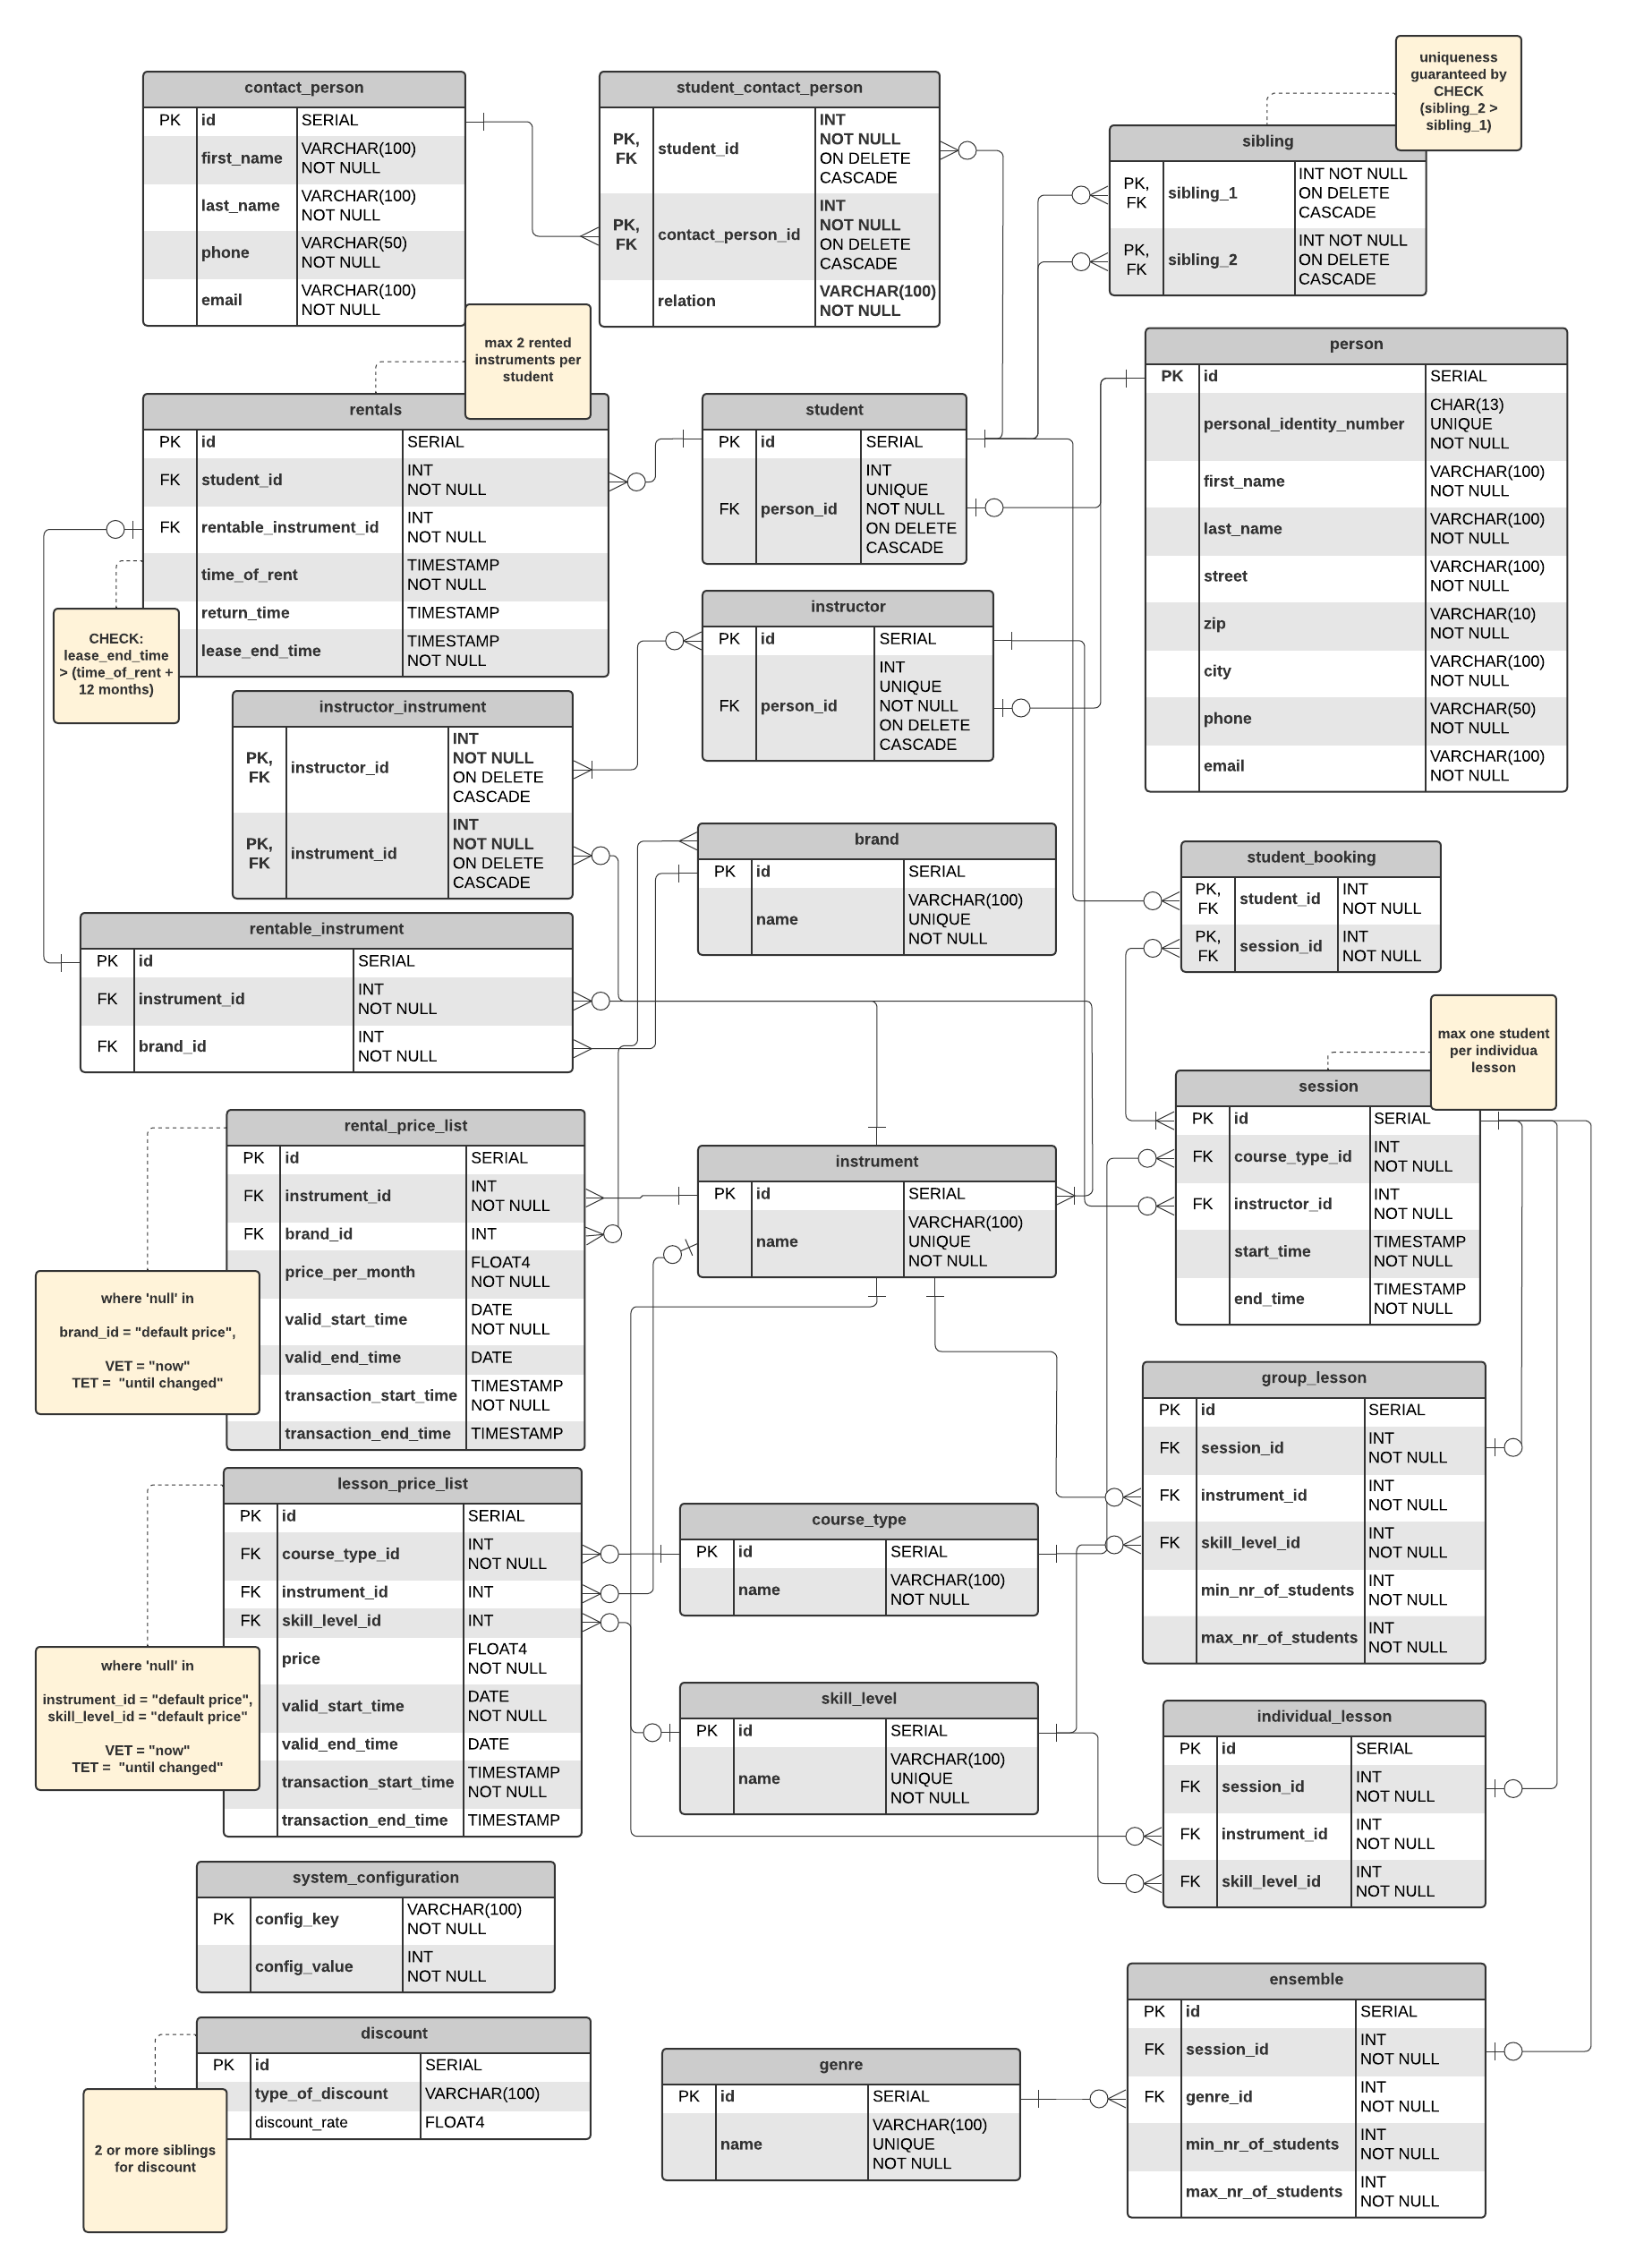
\includegraphics[width=\textwidth]{../figures/logi_phys.png}
    \caption{The Logical and Physical Model using IE notation}
    \label{fig:lpm}
  \end{center}
\end{figure}

\subsection*{Magic numbers}
\label{subsec:magicnumbers}
The table \verb|system_configuration| was created to store configurable parameters,
also known as \emph{''magic numbers''}.
Each row in this table represents a configurable parameter of the system.
The \verb|config_key| column contains a unique identifier for each setting,
and the \verb|config_value| column contains the actual value for that setting.

%\begin{minted}{sql}
%CREATE TABLE system_configuration (
%    config_key VARCHAR(100) PRIMARY KEY,
%    config_value INT NOT NULL
%);
%
%INSERT INTO system_configuration (config_key, config_value)
%VALUES ('max_rentables_per_student', 2),
%       ('min_siblings_for_discount', 2),
%       ('lease_duration_months', 12);
%\end{minted}

\begin{longlisting}
  \inputminted[
    label=Q1-Function,
    linenos=true,
    bgcolor=lightgray,
    firstline=17,
    lastline=20,
%        frame=single,
    fontsize=\footnotesize,
  ]{sql}{../../src/db/tables/create_tables_soundgood_db.sql}
  \caption{The table that stores configurable parameters.}
  \label{listing:sys_config_table}
\end{longlisting}

\begin{longlisting}
  \inputminted[
    label=Q1-VIEW,
    linenos=true,
    bgcolor=lightgray,
    firstline=18,
    lastline=21,
%        frame=single,
    fontsize=\footnotesize,
  ]{sql}{../../src/db/data/populate_tables.sql}
  \caption{Script that populates the system configuration table with current ''magic numbers''.}
  \label{listing:sys_config_pop}
\end{longlisting}

The purpose of this is to keep track of
\begin{itemize}
  \item the minimum number of siblings per student for discount. Currently $2$,
  \item lease duration for renting instruments (currently 12 months) and
  \item the maximum number of instruments a student can rent at a time.
\end{itemize}

When the application starts or when it is in use, it reads from this table to determine the values of various parameters.
For instance, when checking if a student is eligible for a discount,
the application queries this table to find out the current value of \verb|min_siblings_for_discount|.
This allows your application to use dynamic values that can be changed at any time without the need to redeploy or
alter the application code (for further discussion see section \nameref{sec:discussion}).

%-- CONFIGURATIONS
%-- These magic numbers are subject to change or might differ based on business logic,
%-- OPEN ISSUE: the script for creating the system_configuration table fits well
%-- in a schema or database directory within src/, while the script for inserting
%-- configuration keys and values could go into either config/ or a data-seeding
%-- directory within src/, depending on how you view these configurations in the
%-- context of your application setup and deployment.
%INSERT INTO system_configuration (config_key, config_value)
%VALUES ('max_rentables_per_student', 2),
%('min_siblings_for_discount', 2),
%('lease_duration_months', 12);


% \textbf{This chapter explains \textit{the result} of what you did.}

% \textbf{The report must show that you have done the work yourself and that you
% have understood what you have done}, both of these goals are met by carefully
% explaining your solution here in the result chapter, and proving that it meets
% the requirements. \textit{State each requirement that is met} and explain
% \textit{how you met it}. Also include links to your code in your Git
% repository, and include also diagrams, see Figure \ref{fig:diag}, and other
% figures to illustrate your reasoning. All figures must be referenced in the
% text. Ask yourself if the solution is clearly explained, and if the reader
% will understand the application. What would you yourself want to know if you
% read about the application, is that included in the report? More specific
% instructions for the content can be found under each task on the Project page
% in Canvas. 


% VF:
% The naming convention is based on 
% Mozilla's SQL Style Guide. 

% Therefore, \emph{Snake Case}
% (sometimes referred to as underscore case or 
%  snake\_case)
% is used, where each space is replaced with an underscore
% and all letters, including the first letter, is written in lowercase. 

% \begin{figure}[h!]
%   \begin{center}
%     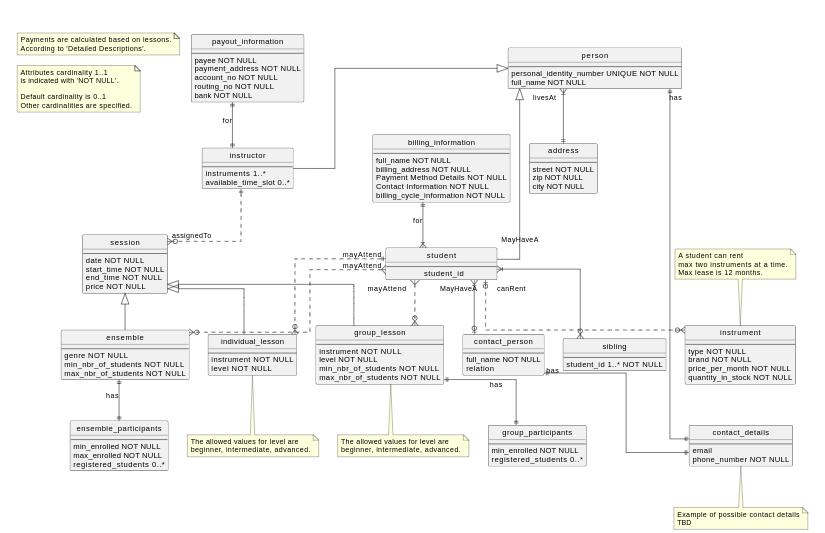
\includegraphics[width=\textwidth]{../figures/i_model.png}
%     \caption{The Conceptual Model with inheritance and payout-/billing information}
%     \label{fig:cm_i}
%   \end{center}
% \end{figure}


\clearpage
\section{Discussion}
  \label{sec:discussion}
The project group justifies the size and complexity of the model (in figure \ref{fig:lpm})
to minimize the reliance on null-values, free-text entries, and enumerated types.

Within the \verb|student| entity, a generated ID functions as the primary key.
Conversely, in the \verb|sibling| entity, a composite key formed from two
student IDs uniquely identifies each sibling pair.
An enforced order in adding siblings eliminates the possibility of duplicate entries
(see the \verb|CHECK| constraint in listing \ref{listing:sibling}).

\begin{longlisting}
  \inputminted[
    label=Q1-Function,
    linenos=true,
    bgcolor=lightgray,
    firstline=83,
    lastline=95,
%        frame=single,
    fontsize=\footnotesize,
  ]{sql}{../../src/db/tables/create_tables_soundgood_db.sql}
  \caption{The table that stores siblings. It includes constraints in order to avoid diplicate entries}
  \label{listing:sibling}
\end{longlisting}

Specific rules for adding siblings, along with guidelines on rental period limits (12 months),
maximum number of rentals per student and sibling discounts,
are added to the model as accompanying note.
A solution is to keep these magic numbers in the \verb|system_configuration| table described in the
\nameref{sec:method} subsection \nameref{subsec:magicnumbers}.

The \verb|contact_person| entity is not linked to the \verb|person| entity in the same manner as
\verb|student| and \verb|instructor| are.
This is because \verb|contact_person| does not require all data present in \verb|person|,
such as personal identity numbers and addresses.

While it was possible to create separate tables for email and phone numbers,
the choice was made against it, under the assumption that these are not typically shared attributes.
Stationary phones are not as common as they used to be.

The combination of the \verb|session| and \verb|student_booking| tables allows multiple students to attend the same session.
The primary key in \verb|student_booking|, a combination of \verb|student_id| and \verb|session_id|,
enables access to session information from all relevant bookings and avoids duplicate bookings.

The use of 'on delete cascade' in certain tables,
like in \verb|sibling|, implies that removing one student from the database would automatically delete the sibling entry,
under the premise that sibling information is irrelevant if both are not registered as students.

\subsection*{Multiple version of data}
Maintaining multiple versions of data in the
\verb|lesson_price_list| and \verb|rental_price_list|
tables enables an accurate historical record of pricing changes.
It provides complete audit trails, useful perhaps for regulatory compliance and internal audits.
In case of disputes or queries about billing, one has a complete historical record to refer to.
This makes it easier to explain and justify charges to students.
Moreover, it ensures data integrity,
which is vital in scenarios involving pricing disputes or the need for data verification.
When prices change mid-semester, the temporal database retains a history of when each price was valid.
This allows the school to invoice students based on the price that was valid at the time of each month's billing period,
even if the price has since changed.

One can perhaps automate the invoicing process to look up the correct price based on the valid time period.
For example, if a student is to be billed for a course or instrument rental, the system can automatically fetch the
price that was valid for the specific month in question.

However, this approach may have disadvantages.
One challenge is the increased need for storage and management capacity due to the additional historical data.
This complexity not only extends to data storage but also may impact the implementation and querying of the tables,
which can become more prone to errors and require more time to manage?
The billing system needs to be capable of understanding and applying these temporal relations.
It must correctly identify and apply the prices that were valid during each billing period.
The author of this report also imagines that larger datasets and complex queries might also lead to performance issues,
impacting the efficiency of database operations.
Furthermore, the maintenance of these tables becomes more challenging,
necessitating more rigorous backup, indexing, etc.

The bi-temporal database approach is well-suited for handling complex invoicing scenarios and the
author of this report is of the belief that it well suited for this project.

\subsubsection*{Future considerations}
Future enhancements to the database may include triggers to ensure that sessions can only be booked if a corresponding price exists,
thereby maintaining data integrity.
These triggers will also regulate that only one student is booked for an individual lesson.

The group considered denormalization for the three types of ''subsessions'' (the two lesson types and ensembles),
due to their similar attributes.
However, this aspect was left open for future discussion and potential implementation.

% \textbf{This chapter \textit{analysis} the result presented in the previous section.} 

% Evaluate your solution according to the assessment criteria found in the assessment-criteria documents, which are found under the bullet \textit{In the Discussion chapter of your report...}, under each task on the Project page in Canvas. You do not have to cover all specified criteria.

\end{document}
